\section*{Cycle 1 Experiment 5 }

\section{\Large{First Readers-Writers Problem}}

\subsection{Aim}
\large To implement the First Readers-Writers Problem.

\subsection{Theory}
The Readers-Writers problem is a classic synchronization problem.\\

\textbf{The problem statement }: There is a shared resource which should be accessed by
multiple processes. There are two types of processes in this context: the reader and
the writer. Any number of readers can read from the shared resource simultaneously,
but only one writer can write to the shared resource. When a writer is writing data
to the resource, no other process can access the resource. A writer cannot write to
the resource if there are non zero number of readers accessing the resource at that
time.\\


\textbf{Solution }: Here, the first reader locks the resource if such is available. Once the file
is locked from writers, it may be used by many subsequent readers without having
them to re-lock it again.\\

Before entering the critical section, every new reader must go through the entry section. However, there may only be a single reader in the entry section at a time so as to avoid race conditions. In order to do so, every reader which enters the ENTRY Section will lock the ENTRY Section for themselves but does not lock the resource. Once the reader is done executing the entry section, it will unlock it by signalling the mutex. There can be no more than a single reader in the exit section at a time, therefore, every reader must claim and lock the Exit section for themselves before using it.\\

Once the first reader is in the entry section, it will lock the resource. Doing this will prevent any writers from accessing it. Subsequent readers can just utilize the locked resource. The very last reader must unlock the resource, thus making it available to writers.

\subsection{Algorithm}
\begin{verbatim}
1 START
2 semaphore resource = NULL;
3 semaphore rmutex = NULL;
4 readcount =0;
5 procedure WRITER
6   resource.P( );
7   <CRITICAL SECTION>
8   <EXIT SECTION>
9   resource.V( );
10 END procedure
11 procedure READER
12  rmutex.P( );
13  <CRITICAL SECTION>
14  readcount++;
15  IF readcount == 1 THEN
16      resource.P( );
17  END IF
18  <EXIT CRITICAL SECTION>
19  rmutex.V( );
20  rmutex.P( );
21  <CRITICAL SECTION>
22  readcount−−;
23  IF readcount == 0 THEN
24      resource.V();
25  END IF
26  <EXIT CRITICAL SECTION>
27  rmutex.v();
28 END procedure
29 STOP
30 . resource.P() is equivalent to wait(resource)
31 . rmutex.P() is equivalent to wait(rmutex)
32 . resource.V() is equivalent to signal(resource)
33 . rmutex.V() is equivalent to signal(rmutex)
\end{verbatim}

\subsection{Program \& Output}
\begin{verbatim}
//First Readers-Writers Problem

#include<pthread.h>
#include<stdio.h>
#include<stdlib.h>
#include<time.h>
#include<unistd.h>

pthread_mutex_t mutex, res;
pthread_t tid;
int readcount = 0;

void *reader(void *var){
    setbuf(stdout, NULL);
    pthread_mutex_lock(&mutex);
    readcount++;
    if (readcount == 1)
        pthread_mutex_lock(&res);\
    printf("Reader %d is inside\n", var);
    pthread_mutex_unlock(&mutex);
    sleep(2);
    pthread_mutex_lock(&mutex);
    readcount--;
    if(readcount == 0)
        pthread_mutex_unlock(&res);
    pthread_mutex_unlock(&mutex);
    printf("Reader is leaving...\n");
    pthread_exit(NULL);
}

void *writer(void *var){
    setbuf(stdout, NULL);
    pthread_mutex_lock(&res);
    printf("Writer has entered\n");
    sleep(2);
    printf("Writer is leaving...\n");
    fflush(stdout);
    pthread_mutex_unlock(&res);
    pthread_exit(NULL);
}

int main(){
    setbuf(stdout, NULL);
    int n1, n2, i, j;
    pthread_mutex_init(&mutex, NULL);
    pthread_mutex_init(&res, NULL);
    srand(time(NULL));
    for(i=0; i<10; i++){
        j = rand();
        if(j%2 == 1)
            pthread_create(&tid, NULL, reader, (void *)i);
        else
            pthread_create(&tid, NULL, writer, NULL);
    }
    pthread_exit(NULL);
}
\end{verbatim}
\begin{figure}[h]
            \centering
            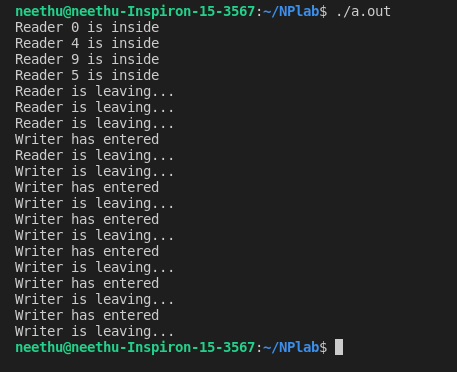
\includegraphics[scale=0.6]{img/e5.png}
\end{figure}

\subsection{Result}
Implemented the program for the first Readers-Writers problem using C language in Ubuntu 20.04 with kernel and the above outputs were obtained.

